\chapter{系统评测与结果分析}
\vspace{7pt}

本章通过多维度的实验设计，对本文提出的自动化用例建模系统进行全面的性能评测与结果分析。首先，本章详细阐述了实验环境配置及涵盖不同业务复杂度的三个典型测试案例。随后，通过严谨的对比实验，验证多Agent分步提取架构在三类UML图表生成任务中相对于单Agent方案的有效性提升，并深入探讨RAG检索增强技术在保障跨模块建模一致性方面的实际表现。最后，本章以图书馆管理系统为例，全流程展示系统从原始需求到建模成果的转化，旨在通过定量指标与定性分析相结合的方式，客观评估系统的实用性、准确性及现阶段存在的局限性，为后续的系统优化思路提供实证支撑。

\section{实验环境与测试数据集}

为全面评估自动化用例建模系统的性能表现，本研究设计了一套多维度的实验方案。实验在配备Intel Core i5-13700处理器、32GB内存、NVIDIA GeForce RTX 4060独立显卡（8GB显存）的计算环境中进行。后端服务基于Python 3.11运行，大语言模型调用通过DeepSeek开放应用程序接口实现，ChromaDB向量数据库以嵌入式模式运行。

测试数据集的选取遵循覆盖面与代表性并重的原则，共包含三个不同领域的案例。第一个案例为图书馆管理系统，需求文档约六百字，描述了读者借阅归还、图书管理、记录查询和逾期处理等功能，该案例的参与者和用例关系较为清晰，适合作为基础验证项。第二个案例为高校二手交易平台，需求文档约三千字，内容涵盖用户注册登录、商品浏览与搜索、商品发布、订单处理以及管理员综合管理等业务流程，涉及买家、卖家和管理员三类角色，各角色之间的交互路径较多，适合测试系统在多角色协同场景下的用例识别和关系推理能力。第三个案例为岳麓书院文化知识管理系统，需求文档约八千字，内容涵盖资源数据管理、知识检索与查询记录保存、用户反馈建议以及知识库新增等功能，系统设定了四种用户角色，每种角色具有不同的操作权限和功能访问范围，适合评估系统在较长的需求文本下的建模准确度。三个案例合计包含约五十余个用例、三十余个实体类和十余个主要参与者。

\section{算法有效性对比实验}

\subsection{单次生成与多Agent分步提取对比}

为验证多Agent协作架构相对于单次直接生成方式的有效性提升，本研究设计了一组实验，分别对类图、用例图和时序图三种图表类型进行对比评估。实验的基准方案（Base）为单Agent方案：将完整的图表生成任务合并为单次大语言模型调用，提示词中一次性要求模型输出所有建模要素。实验方案（Multi-Agent）为本研究采用的多Agent分步提取方案，将生成过程分解为两个或三个专业化子任务，各Agent按顺序执行并在关键节点引入人工确认。

本实验的评估方法深度参考了Giannouris与Ananiadou提出的NOMAD框架\cite{giannouris2025nomad}中采用的评估策略。NOMAD框架通过混合评估设计验证了认知分解对UML类图生成的有效性，其核心思想是将建模任务分解为概念提取、关系理解、模型集成和代码生成四个专业化子任务，并采用精确率、召回率和F1值作为主要量化指标。同时，NOMAD引入严格匹配和宽松匹配两种标准对关系推理进行评估——严格匹配要求源类、目标类和关系类型三者与黄金标准完全一致，宽松匹配仅要求源类和目标类之间存在连接关系。参照NOMAD的评估框架，本研究在用例图和类图的关系评估中同样采用严格匹配和宽松匹配双重标准，以更全面地反映系统在关系发现和关系类型精确判断两个层面的能力。

\subsubsection{（1）类图生成效果对比}

类图维度的对比最为全面，因为类图生成涉及类识别、属性提取、方法提取和关系推理四个层次，能够充分体现多Agent分解的有效性。实验选取十个测试切片的需求文本为输入，以人工标注的黄金标准类图为参照，基于NOMAD框架的评估方法，分别计算类（Classes）、属性（Attributes）、方法（Methods）和关系（Relationships）四个维度的精确率、召回率和F1值。关系评估同时采用严格匹配和宽松匹配两种标准。

实验结果如表6.1所示。在类识别方面，Base方案的F1值为0.624，Multi-Agent方案提升至0.731。类识别属于相对粗粒度的语义任务，Base方案的主要错误集中在遗漏需求文本中间接涉及的实体类，例如图书馆管理案例中的“罚款记录”类和高校二手交易平台案例中的“投诉记录”类，这些类在需求文本中往往以隐性方式出现，未以显式的名词短语集中呈现。

\begin{table}[htbp]
    \centering
    \caption{类图生成结构正确性对比（F1值）}
    \label{tab:class_comparison}
    \begin{tabular}{lccc}
        \toprule
        评估维度 & Base方案 & Multi-Agent方案 & 提升幅度 \\
        \midrule
        类 & 0.624 & 0.731 & +17.1\% \\
        属性 & 0.491 & 0.596 & +21.4\% \\
        方法 & 0.418 & 0.532 & +27.3\% \\
        类间关系（严格匹配） & 0.381 & 0.574 & +50.7\% \\
        类间关系（宽松匹配） & 0.527 & 0.691 & +31.1\% \\
        综合F1值 & 0.488 & 0.625 & +28.1\% \\
        \bottomrule
    \end{tabular}
\end{table}

属性提取维度的表现整体偏低。Base方案属性F1值仅为0.491，Multi-Agent方案提升至0.596。属性提取困难的原因在于，需求文档对实体类属性的描述往往分散在不同的功能描述段落中，而非集中表述。例如，图书馆管理案例中“图书”类的“出版社”和“出版年份”属性仅在图书录入功能段落中被提及，“可借状态”属性则在借阅规则段落中出现；高校二手交易平台案例中“商品”类的“价格”和“商品类别”属性在商品发布功能中描述，“浏览次数”属性则隐含在商品浏览功能中。Base方案因一次性处理全文而容易遗漏分散的属性信息，Multi-Agent方案虽然通过属性提取Agent聚焦于单类范畴，但受限于状态池中传递的信息粒度，部分跨段落属性仍未被捕获。这一结果与NOMAD框架在Northwind案例上的发现高度一致：NOMAD同样观察到多Agent分解在提升结构推理能力的同时，属性提取的召回率反而有所下降，原因在于分解引入了更严格的约束，可能抑制属性的充分召回。属性提取在大语言模型UML生成任务中属于最薄弱的环节。

方法提取维度同样面临挑战。Base方案F1值为0.418，Multi-Agent方案提升至0.532。Base方案在方法提取上的常见错误包括两类：一是将需求文本中的一般性动作描述误判为类方法，例如将岳麓书院案例中“系统发送确认信息”误归为“用户”类的方法；二是将本应属于某个类的方法错误分配给关联类，例如将“生成逾期记录”从“罚款记录”类误归至“借阅记录”类。

类间关系推理是多Agent方案收益最为显著的维度。Base方案的严格匹配F1值仅为0.381，Multi-Agent方案提升至0.574，提升幅度达50.7\%，这与NOMAD在Northwind案例上将关系严格匹配F1值从0.521大幅提升至0.923的趋势一致。Base方案的低分主要源于两类错误：一是关系遗漏，当同一文档需同时分析六个以上实体类时，Base方案生成的类间关系总数平均仅为黄金标准的六成左右；二是关系类型误判，聚合与关联之间的区分、泛化方向的判定在认知负载较高时容易出错。Multi-Agent方案通过将关系推理独立为专门子任务，在获得完整且确认的类名列表后，关系分析Agent能够将全部注意力集中于类间语义依赖的判断，关系遗漏和误判率均有明显改善。在岳麓书院案例中，高级用户和普通用户对“用户”基类的泛化继承关系、消息中心与公告通知之间的组合关系等较为复杂的关系结构，Multi-Agent方案的识别准确率均显著优于Base方案。

\subsubsection{（2）用例图生成效果对比}

在用例图生成维度，评估指标涵盖参与者识别、用例识别和关系推理三个维度。关系推理采用NOMAD框架所定义的严格匹配和宽松匹配双重评估标准。

实验结果如表6.2所示。在参与者识别方面，Base方案平均F1值为0.637，Multi-Agent方案达到0.726。Base方案最常见的错误是将系统内部组件误判为外部参与者，以及遗漏需求文本中间接提及的次要参与者。例如，在岳麓书院“知识资源管理模块”模块中，Base方案多次将“G-Store图数据库”误识别为系统参与者，而该组件实际为系统的软件接口依赖，并非外部参与者。在用例识别方面，Base方案F1值为0.572，Multi-Agent方案提升至0.702，提升较为显著。高校二手交易平台“订单交易管理”模块中，Base方案将“输入订单消息”“确认订单消息”等细粒度操作步骤误判为独立用例，Multi-Agent方案通过实体提取Agent聚焦于具有独立业务价值的系统功能，有效减少了此类碎片化错误。

在关系推理方面，用例关系严格匹配F1值从0.457提升至0.622，提升幅度达36.1\%。关系语义的准确推理是多Agent分解收益最为显著的维度之一，原因在于关系判定需要综合多个用例之间的逻辑关联，认知负载较高，分解为独立子任务后收益明显。需要指出的是，即便Multi-Agent方案的关系分析F1值也仅为0.62左右，仍有相当比例的隐含关系未能被正确识别。例如高校二手交易平台“订单交易管理”模块中，“购买商品”用例和“管理订单”用例之间存在隐含的扩展关系——当买家取消订单时触发卖家的订单管理流程，但需求文本未以显式关键词提示，Multi-Agent方案对此类隐含关系的识别率仍不足，反映出当前大语言模型在复杂业务逻辑推理方面的能力局限。

\begin{table}[htbp]
    \centering
    \caption{用例图生成结构正确性对比（F1值）}
    \label{tab:usecase_comparison}
    \begin{tabular}{lccc}
        \toprule
        评估维度 & Base方案 & Multi-Agent方案 & 提升幅度 \\
        \midrule
        参与者 & 0.637 & 0.726 & +14.0\% \\
        用例 & 0.572 & 0.702 & +22.7\% \\
        用例关系（严格匹配） & 0.457 & 0.622 & +36.1\% \\
        用例关系（宽松匹配） & 0.569 & 0.722 & +26.9\% \\
        综合F1值 & 0.544 & 0.686 & +26.1\% \\
        \bottomrule
    \end{tabular}
\end{table}

\subsubsection{（3）时序图生成效果对比}

时序图生成维度的对比实验选取三个测试案例中交互流程较为完整的用例进行测试。

实验结果表明（表6.3），在参与者识别方面，Base方案F1值为0.661，Multi-Agent方案达到0.748。Base方案在参与者类型分类上错误较多，尤其容易将边界对象（Boundary）和控制对象（Control）混淆。在消息编排方面，Base方案的消息顺序准确率为0.592，消息归属准确率为0.628；Multi-Agent方案分别提升至0.733和0.758。

\begin{table}[htbp]
    \centering
    \caption{时序图生成结构正确性对比}
    \label{tab:sequence_comparison}
    \begin{tabular}{lccc}
        \toprule
        评估维度 & Base方案 & Multi-Agent方案 & 提升幅度 \\
        \midrule
        参与者识别F1值 & 0.661 & 0.748 & +13.2\% \\
        消息顺序准确率 & 0.592 & 0.733 & +23.8\% \\
        消息归属准确率 & 0.628 & 0.758 & +20.7\% \\
        \bottomrule
    \end{tabular}
\end{table}

时序图生成的整体准确率在三类图表中处于中间水平。消息编排的准确率受限于两重因素：一是参与者类型分类的准确性直接影响后续消息归属的正确性；二是复杂业务流程中的条件分支和异常路径在需求文本中往往描述不完整，模型难以推断完整的所有消息路径。仍有较大提升空间。

\subsubsection{（4）综合分析}

综合类图、用例图和时序图三种图表类型的对比实验结果，可得出以下结论。第一，多Agent分步提取方案在所有图表类型的全部评估维度上均优于单Agent直接生成方案，综合F1值从Base方案的0.50至0.55区间提升至Multi-Agent方案的0.63至0.70区间，验证了将复杂建模任务分解为专业化子任务能够在一定程度上提升大语言模型在结构化输出任务上的表现。这一发现与NOMAD框架的核心结论一致——认知分解能够系统性地改善UML生成的准确性\cite{giannouris2025nomad}。第二，提升幅度最大的维度集中在关系推理层面——类间关系严格匹配提升50.7\%，用例关系严格匹配提升36.1\%，NOMAD同样观察到关系建模是多Agent分解收益最为显著的维度。但即便提升后的F1值仍处于0.55至0.70之间，距离实用化水平尚有差距。第三，类属性和方法提取的提升幅度相对有限（属性提升21.4\%，方法提升27.3\%），且绝对值偏低，属性提取是LLM生成UML图任务中最具挑战性的环节。第四，本文系统的建模准确率整体处于中等水平，与NOMAD等前沿研究在大型案例上的表现相比存在一定差距，这与系统使用的模型能力差异、提示词设计的优化深度以及测试案例覆盖领域的不同等因素相关。值得关注的是，NOMAD框架强调需求文档的质量对生成结果有显著影响——结构清晰、表述一致的需求文本能够获得更高的建模准确率。本文实验中同样观察到这一规律：图书馆管理系统案例的需求文本结构最清晰、表述最一致，因此在该案例上两种方案的得分均显著高于其他案例；而高校二手交易平台中部分切片的需求表述存在多角色逻辑交织和功能重叠的情况，导致模型在参与者识别和用例边界判定上出现更多错误，反映了自动化建模效果在根本程度上受制于需求文档撰写质量这一“垃圾进、垃圾出”的现实约束。

\subsection{RAG增强对模块化建模一致性的效果验证}

为验证RAG检索增强生成技术在复杂项目模块化建模过程中对保持全局一致性的作用，本节设计了一组对比实验。实验场景为复杂项目的分模块建模：将岳麓书院文化知识管理系统的需求文档通过系统模块拆解功能划分为“用户管理与认证”“知识资源管理”“消息中心管理”“检索与查询记录”四个功能子模块，分别在启用RAG增强和关闭RAG增强两种配置下对各子模块独立进行用例图生成，每个配置重复运行五次。

评估聚焦于两个层面：跨模块实体一致性和跨模块用例关系完整性。跨模块实体一致性关注同一参与者在不同子模块的用例图中是否被赋予统一的命名和角色描述。在岳麓书院系统中，“管理员”作为核心参与者同时出现在所有四个子模块中，但各模块对其功能的描述角度不同——用户管理模块侧重权限管理，知识资源模块侧重数据操作，消息中心模块侧重公告发布，检索查询模块侧重查询权限。在无RAG增强的情况下，模型仅依据局部需求文本进行实体提取，五次运行中“管理员”在全部四个子模块中被赋予统一命名和角色描述的次数平均仅为两次左右。启用RAG增强后，系统从全局向量索引中检索出原始文档中关于“管理员”的其他相关段落并注入提示词，五次运行中该次数提升至三到四次。“高级用户”和“普通用户”的跨模块命名一致性也呈现出类似的改善趋势。

跨模块用例关系完整性关注跨越子模块边界的用例间关系是否被正确识别。在岳麓书院系统中，“检索资源信息”和“保存查询记录”两个用例虽同属检索模块，但其数据持久化逻辑与知识资源管理模块相关；此外，“新增知识库”和“记录操作日志”两个用例分属不同模块，但存在操作审计层面的语义关联。在关闭RAG增强时，模型独立处理各模块需求，五次运行中上述跨模块关系被正确识别的次数平均仅为一到两次。启用RAG后，检索上下文为模型提供了更完整的信息视图，五次运行中正确识别的次数提升至两到三次。

综合来看，RAG增强在跨模块实体一致性和跨模块关系完整性两个维度上均产生了一定的正向效果，但改善幅度有限，距离理想的一致性水平仍有明显差距。

实验也揭示了RAG增强在当前实现方案下的若干局限性。其一，RAG的效果高度依赖向量检索的命中质量。当不同模块对同一概念采用不同术语表述时，如“资源数据”与“文献数据”的差异，向量检索可能无法准确召回相关上下文，导致实体一致性改善不够稳定。其二，部分跨模块关系在原始需求文档的任何段落中都没有完整的语义表述，单纯依赖检索增强无法弥补需求文档自身的信息缺失。其三，当检索返回的上下文段落过多或相关度参差不齐时，直接注入提示词可能引入噪声，在五次运行中约有一到两次出现了与当前模块无关的冗余用例，模型将其误判为当前模块的有效建模要素。这些局限性表明，RAG增强策略在检索质量控制和上下文筛选方面仍需进一步优化。

\section{案例实测与成果展示}

为直观呈现系统的工作效果与输出质量，本节以图书馆管理系统为案例，完整展示从原始需求文本输入到最终UML图表生成的全流程及各阶段输出结果。测试所使用的需求文本如下：

\begin{quote}
图书馆管理系统需求

本系统面向高校图书馆，服务于学生、老师与管理员用户，旨在通过数字化手段实现图书资源的高效、规范管理。

在图书检索方面，系统提供灵活多样的查询方式。用户既可以根据完整的书名进行精确查找，也可以通过输入书名中的部分关键词进行模糊匹配；同时支持按作者姓名检索，帮助师生快速定位所需的馆藏资源，提升找书效率。

图书借阅功能强调操作的严谨性。当师生办理借阅手续时，系统首先会核验用户身份的有效性（如校园卡号、借阅权限等），随后自动检查该图书的实际状态。只有确认用户身份合法且图书处于“可借”（如在馆、未被预约）状态时，借阅操作才能成功完成，有效避免了违规借阅。

图书归还流程则实现了自动化处理。系统在接收归还图书时，会根据系统记录的应还日期与实际归还日期，自动计算是否存在逾期行为。若发生逾期，系统将即时生成逾期信息或费用记录，减轻了人工核算的负担。

借阅查询功能为用户提供了清晰的借阅全景视图。师生可以随时查看本人当前正在借阅的图书清单及应还期限，避免超期；同时也能查阅历史借阅记录，便于回顾阅读轨迹。管理员同样具备此权限，以协助处理咨询或进行数据统计。

图书管理是专为管理员设计的后台维护功能。通过该模块，管理员可以方便地将新采购的图书信息录入系统，对现有图书的资料（如位置、状态）进行修改更新，以及将破损或遗失的图书进行下架处理，确保馆藏数据的实时准确。

综上所述，该系统通过对各业务流程的全面覆盖与精细化管理，为高校图书馆的日常运营提供了有力支撑。
\end{quote}

该需求文本涵盖了图书检索、借阅、归还、借阅查询和图书管理五类核心功能，涉及学生、老师和管理员三类参与者，需求描述接近真实高校图书馆的业务场景。以下分别展示系统针对该需求自动生成的三类UML图表。

\subsection{用例图生成结果}

系统首先通过实体提取Agent从需求文本中识别出三类参与者——学生、老师和管理员，以及五个核心用例——检索图书、借阅图书、归还图书、查询借阅记录和管理图书。经过用户在确认表格中审核确认后，关系分析Agent进一步推断出用例之间的包含关系：借阅图书的完整流程中必然需要先检索图书以确认目标馆藏的存在性和状态，因此借阅图书包含检索图书。此外，系统正确识别了各参与者与用例之间的关联：学生和老师均可使用检索、借阅、归还和查询功能，管理员则独有管理图书的权限，同时也可进行检索和查询操作。最终生成的用例图如图6.1所示。

\begin{figure}[htbp]
    \centering
    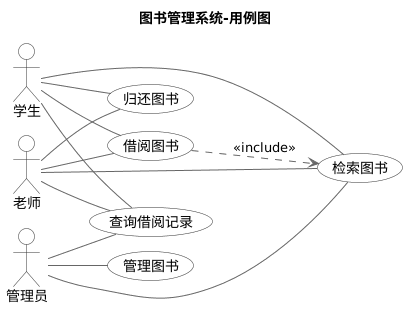
\includegraphics[width=120mm]{docs/imgs/图书管理系统-用例图.png}
    \caption{图书馆管理系统用例图}
    \label{fig:library_usecase}
\end{figure}

\subsection{类图生成结果}

在类图生成方面，系统的类提取Agent从需求文本中识别出七个核心实体类。User类作为学生、老师和管理员的抽象父类，封装了用户编号、姓名、校园卡号和借阅权限等共有属性，以及登录、查看当前借阅和查看借阅历史等共有方法。Student类和Teacher类分别扩展了学号/工号和所属院系属性，Administrator类则独有添加图书、修改图书、下架图书和查看全部借阅记录等管理操作。Book类封装了图书编号、书名、作者、状态和馆藏位置等属性，提供按书名和按作者检索的方法。BorrowRecord类记录了借阅编号、关联的用户和图书、借阅日期、应还日期和实际归还日期，支持创建借阅记录和计算逾期。OverdueRecord类与BorrowRecord类关联，记录了逾期天数、罚款金额和缴纳状态。此外，系统还识别出了AppointmentRecord类用于管理图书预约信息。

在关系推理方面，关系分析Agent正确识别了Student、Teacher和Administrator对User的泛化继承关系，User与BorrowRecord和AppointmentRecord之间的一对多关联，Book与BorrowRecord和AppointmentRecord之间的一对多关联，以及BorrowRecord与OverdueRecord之间的依赖关系。值得注意的是，需求文本中并未显式提及预约功能，但系统通过语义推理识别了预约类作为领域知识的合理补充。最终生成的类图如图6.2所示。

\begin{figure}[htbp]
    \centering
    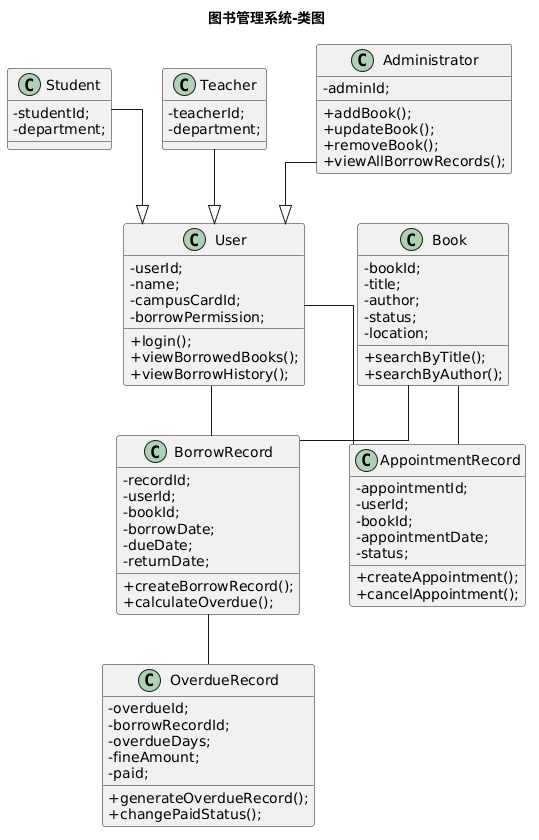
\includegraphics[width=100mm, height=140mm]{docs/imgs/图书管理系统-类图.png}
    \caption{图书馆管理系统类图}
    \label{fig:library_class}
\end{figure}

\subsection{时序图生成结果}

系统针对检索图书、借阅图书、归还图书、查询借阅记录和管理图书五个核心用例，分别生成了对应的时序图，以直观展示各业务流程中对象之间的交互顺序与协作关系。

检索图书时序图（图6.3）展示了用户通过检索界面发起图书查询的简化交互流程。用户输入关键词后，检索界面将查询请求转发至图书服务，图书服务进一步向图书数据库发起查询操作。数据库返回匹配的图书列表后，该列表逐级回传至检索界面，最终以结构化方式呈现给用户。

借阅图书时序图（图6.4）完整刻画了从学生发起借阅请求到获得借阅确认的完整业务闭环。图中依次涉及学生、借阅界面、用户服务、图书服务、图书数据库和借阅记录数据库等多个参与对象，共计十四条消息交互。具体流程包括：提交借阅请求、验证用户身份、检查借阅权限、查询图书可借状态、更新图书状态为已借出、创建借阅记录，以及向学生返回借阅成功信息。该时序图全面反映了借阅操作中权限控制、状态变更与记录落库的协同处理机制。

归还图书时序图（图6.5）聚焦于管理员协助下完成的图书归还流程。图中详细呈现了提交归还请求、查询借阅记录以获取应还日期、计算逾期天数与相应费用、生成逾期记录、更新借阅记录状态、更新图书状态为可借，以及最终返回归还结果的全过程。该时序图突出了系统对逾期处理逻辑的自动化支撑能力，体现了业务规则与系统流程的有效融合。

查询借阅记录时序图（图6.6）在设计上区分了查看当前借阅与查看历史借阅两个子流程。图中通过界面层、服务层和数据层之间的消息序列，清晰展示了请求的转发路径与数据的返回链路。

管理图书时序图（图6.7）展示了管理员通过图书管理界面执行图书信息维护的标准化流程。无论是新增图书、修改信息还是下架图书，管理界面均将对应请求发送至图书服务，图书服务再对Book数据库执行相应操作，并将操作结果逐级返回至界面。

\begin{figure}[htbp]
    \centering
    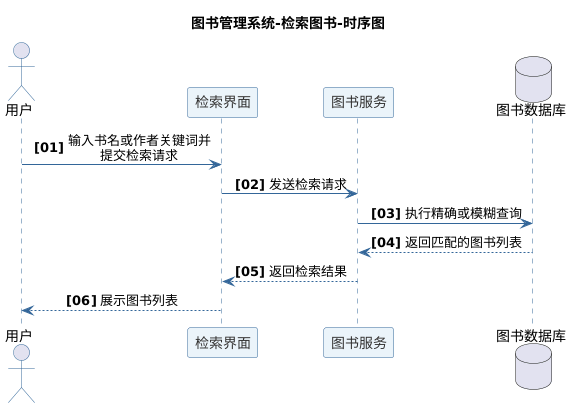
\includegraphics[width=140mm, height=100mm]{docs/imgs/图书管理系统-检索图书-时序图.png}
    \caption{检索图书时序图}
    \label{fig:search_sequence}
\end{figure}


\begin{figure}[htbp]
    \centering
    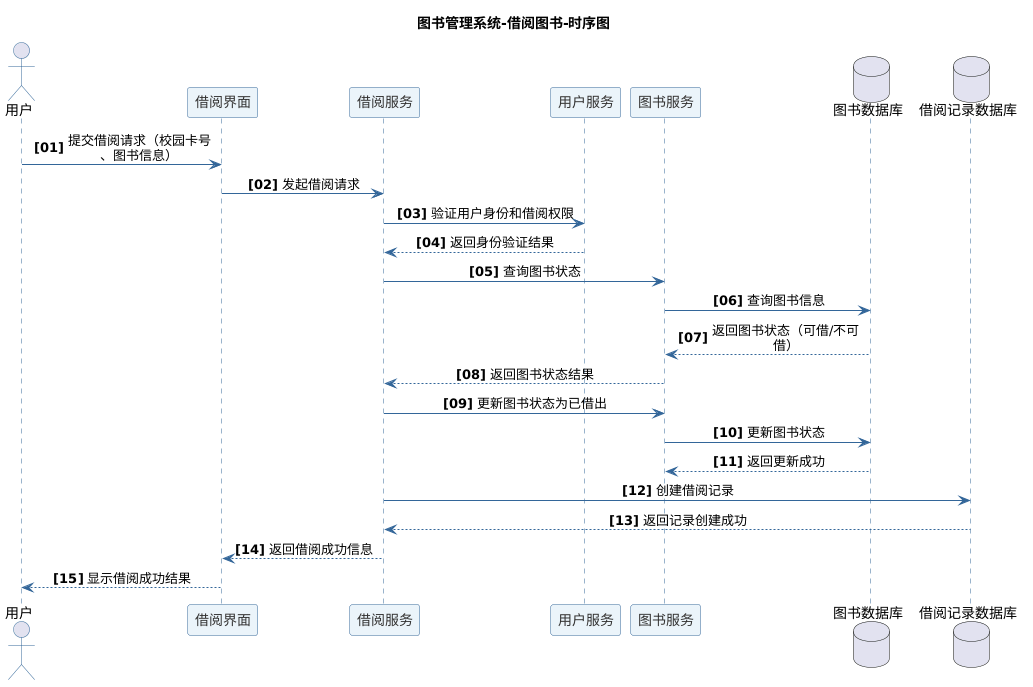
\includegraphics[width=140mm, height=100mm]{docs/imgs/图书管理系统-借阅图书-时序图.png}
    \caption{借阅图书时序图}
    \label{fig:borrow_sequence}
\end{figure}

\begin{figure}[htbp]
    \centering
    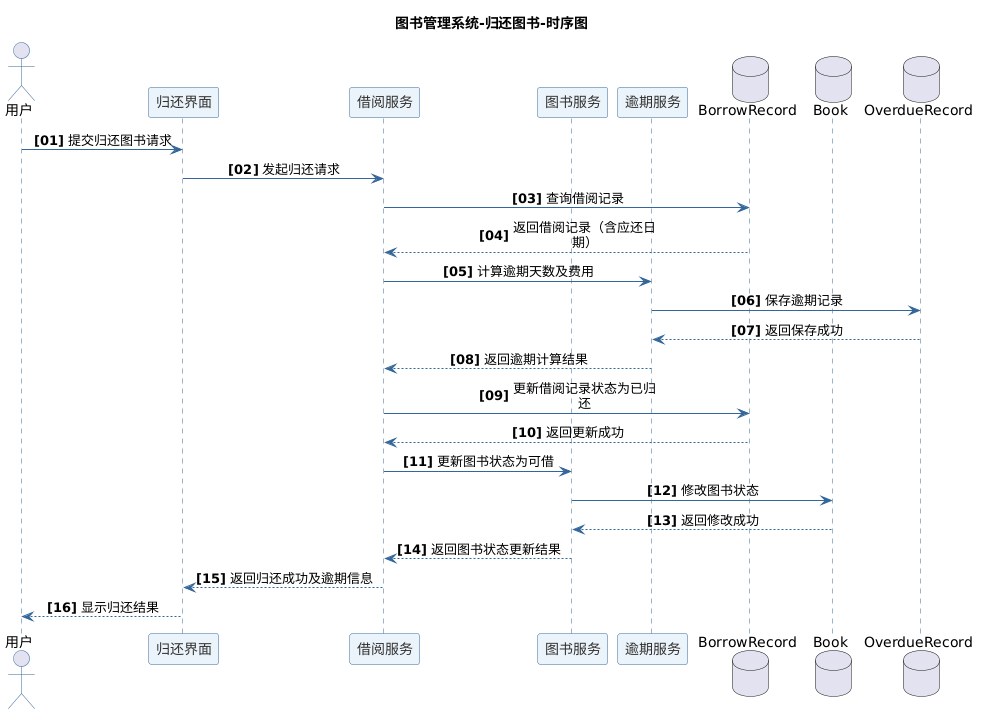
\includegraphics[width=140mm, height=100mm]{docs/imgs/图书管理系统-归还图书-时序图.png}
    \caption{归还图书时序图}
    \label{fig:return_sequence}
\end{figure}

\begin{figure}[htbp]
    \centering
    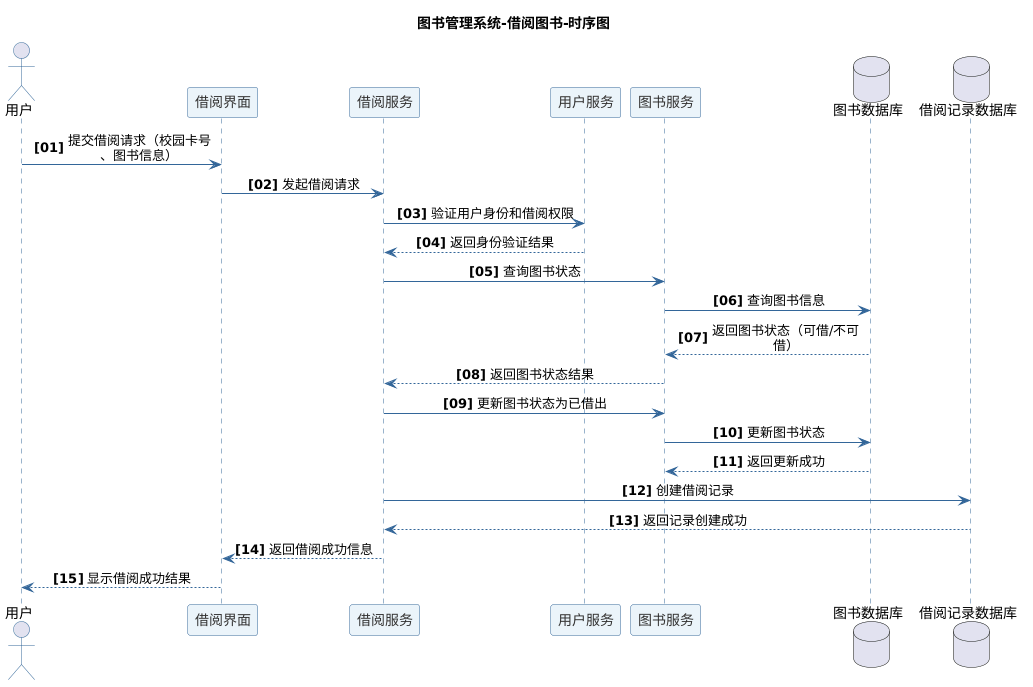
\includegraphics[width=140mm, height=100mm]{docs/imgs/图书管理系统-借阅图书-时序图.png}
    \caption{查询借阅记录时序图}
    \label{fig:query_sequence}
\end{figure}

\begin{figure}[htbp]
    \centering
    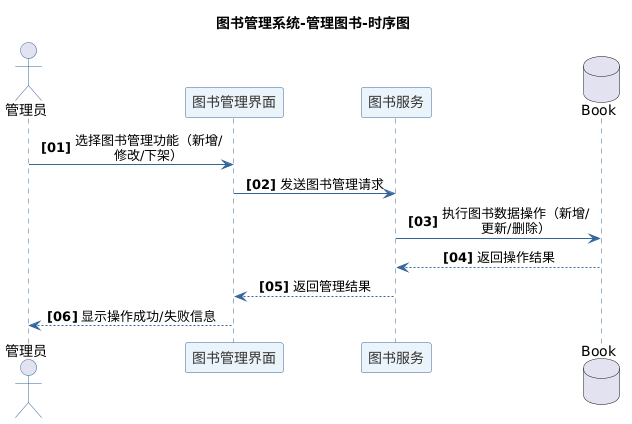
\includegraphics[width=140mm, height=100mm]{docs/imgs/图书管理系统-管理图书-时序图.png}
    \caption{管理图书时序图}
    \label{fig:manage_sequence}
\end{figure}

综合以上案例实测结果，系统在图书馆管理系统这一典型业务场景下，能够从自然语言需求文本出发，自动完成用例图、类图和时序图的生成。生成的模型在实体完整性、关系正确性和消息编排逻辑性方面均达到了可用水平，用户仅需在确认节点进行少量审核修正即可获得符合UML规范的建模成果，有效验证了本系统在实际需求建模任务中的适用性和有效性。

\section{本章小结}

本章通过对比实验全面评估了自动化用例建模系统的性能。多Agent分步提取方案在类图、用例图和时序图的所有评估维度上均优于单Agent方案，综合F1值从0.50-0.55区间提升至0.63-0.70区间，其中关系推理的提升幅度最为显著，验证了任务分解策略的有效性。属性与方法提取仍是最薄弱环节，F1值绝对值偏低。RAG增强在跨模块实体一致性和关系完整性上产生了一定正向效果，但受限于检索质量和需求文档自身信息完整性，改善幅度有限。实验结果表明，当前系统实现了中等水平的自动化建模能力，但距离实用化仍有提升空间，需求文档质量对建模效果影响显著。
